\section{Revised Block Diagram}

Figure~\ref{fig:blockDiagram} shows a revised system block diagram.  It contains the model numbers of the known components, the type of connection required to the microcontroller unit and the amount of lines needed for each connection.  Several components such as the power management circuit, battery meter and charger are still to be chosen as several methods of battery charging are being considered.

%TODO Fix amount of lines in block diagram
\begin{figure}[H]
	\centering
	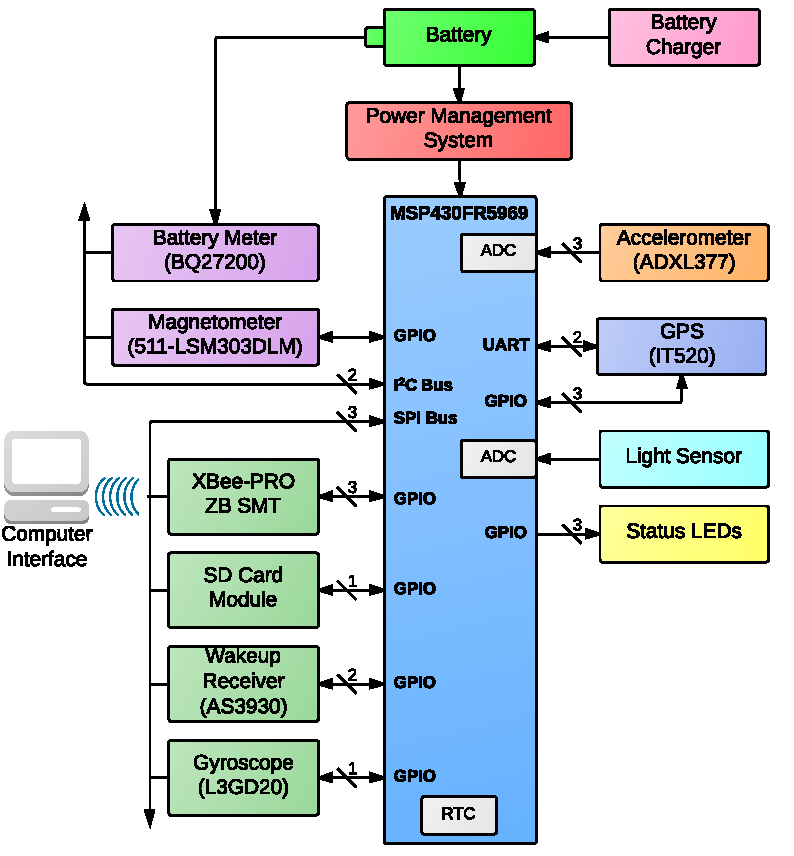
\includegraphics[width=\textwidth]{img/blockDiagramV2_2}
	\caption{Revised Block Diagram \label{fig:blockDiagram}}
\end{figure}

\subsection{Battery Charging Methods}
\subsubsection{USB Charger}
Big effort has been made in recent years to standardize chargers and connectors for music players, cellphones, tablets, and many other consumer electronic products. Micro USB has taken the lead as the standard port for charging consumer electronics and manufacturers have dropped their own proprietary connectors to favor the USB standard.
The USB 2.0 standard included the Battery Charging Specification 1.2, which increased the limits of supply current to 1.5A, up from the 500mA the USB 1.0 standard allowed. The USB 3.0 specification allows 900mA of current drawn while concurrently transmitting data. For battery charging, the limit is still 1.5A, even though the Battery Charging specification requires the physical ports themeselves to be able to handle 5A.
There are many variables in question when it comes to choosing a battery charger. Different battery technologies need to be charged distinctively. For this application, a technology such as Lithium-Ion or Lithium-Polymer must be used, because Lead-Acid, Nickel-Cadmium, and Nickel-Metal-Hydride batteries are too big, heavy, and do not provide the necessary voltage for this application. It is for this reason also that Li-Ion and Li-Polymer batteries are chosen for most consumer electronics.
Other variables include the number of battery cells that need to be charged and the kind of topology needed to charge the battery. For Lithium-Ion and Lithium-Polymer, two topologies exist: Linear and Switch-mode.
Most handheld devices use a linear charging topology, because it offers many advantages like low implementation cost, design simplicity, and a non-noisy operation because it has no high frequency switching components. One of the drawbacks of this topology is that it introduces power dissipation in the system. Switch-mode topology offers higher efficiency, but the implementation is more complicated, bulkier, and noisy, which may cause interference. For this application, a linear charging topology is preferred.
After having decided the implementation variables, a charge management controller should be chosen. There are many controllers available commercially. A good example is Microchip's MCP73831/2. This is a single cell, fully integrated Li-Ion and Li-Polymer charge management controller. It uses a linear topology and it is compatible with the stardard Micro USB port. 
Another good example is Texas Instrument's bq24080. It also uses a linear charge topology, and contains a status indicator pin.
\subsubsection{Wireless Charger}
